\documentclass[10pt]{article}
\usepackage[T1]{fontenc}
\usepackage[utf8]{inputenc}
\usepackage[polish]{babel}
\usepackage{amsthm}
\usepackage{amsfonts}
\usepackage{titlesec}
\usepackage{graphicx}
\title{%
  Sprawozdanie \\
  \large P2.16 z analizy numerycznej\\
    obliczanie i badanie wielomianu $s_{n}(x) = \sum_{k=0}^{'n} c_{k} T_{k}(x)$}
\author{Mateusz Markiewicz}
\begin{document}
\maketitle
\tableofcontents

\newtheorem{definition}{Definicja}[section]

\titleformat{\paragraph}
{\normalfont\normalsize\bfseries}{\theparagraph}{1em}{}
\titlespacing*{\paragraph}
{0pt}{3.25ex plus 1ex minus .2ex}{1.5ex plus .2ex}

%~~~~~~~~~~~~~~~~~~~~~~~~~~~~~~~~~~~~~~~~
\newpage
\section{Wstęp}
\subsection{Cel zadania}

Celem zadania jest skonstruowanie szybkiego oraz numerycznie poprawnego algorytmu obliczającego wartość wielomianu $s_{n}$ w punkcie $x$, gdzie \\
$s_{n}(x) := \sum_{k=0}^{'n} c_{k} T_{k}(x)$, a $T_{k}(x)$ oznacza k-ty wielomian Czebyszewa.

\subsection{Streszczenie sprawozdania}
Po wstępie teoretycznym do omawianego zagadnienia przedstawię algorytm Clenshowa oraz jego wersję dla wielomianów Czebyszewa oraz pokażę, jak można wykorzystać go do wyznaczenia wartości sumy $s_{n}(x) = \sum_{k=0}^{'n} c_{k} T_{k}(x)$. Następie pokażę przykłady dokładności oraz numerycznej poprawności zaproponowanego rozwiązania.

\section{Opis teoretyczny problemu}
\subsection{Wprowadzenie do zagadnienia}
Dowolny wielomian $w_{n}(x)$ możemy przedstawić w bazie wielomianów Czebyszewa, czyli jako kombinację liniową w postaci $\sum_{k=0}^{'n} c_{k} T_{k}(x)$. \\
Wielomiany Czebyszewa są układem wielomianów ortogonalnych, stąd tworzą one bazę dla przestrzeni wielomianów. Zdefiniowane są w następujący rekurencyjny sposób:
\begin{center}
$T_{0}(x) := 1, \: T_{1}(x) := x$ \\
\vspace{0.2em} $T_{k}(x) := 2x T_{k-1}(x) - T_{k-2}(x)$
\end{center}
Korzystając jednak z powyższej zależności rekurencyjnej do obliczenia wartości wielomianu $w_{n}$ punkcie $x$ (zakładając, że korzystamy z definicji $w_{n}$ w postaci kombinacji liniowej wielomianów Czebyszewa) byłoby możliwe w czasie wykładniczym względem $n$. \\
Powyższe obserwacje prowadzą do wniosku, że potrzebny jest inny algorytm służący do obliczania wartości sumy $\sum_{k=0}^{'n} c_{k} T_{k}(x)$. Algorytm ten musi spełniać nie tylko założenia czasowe, ale musi być również numerycznie poprawny. \\ 

Zgodnie z książką \textit{,,Analiza Numeryczna'', D.Kincaid, W.Cheney} algorytm jest numerycznie poprawny (numerycznie stabilny), jeśli dla lekko zaburzonych danych zwraca lekko zaburzony wynik. \\

Zapamiętując 2 poprzednie wielomiany Czebyszewa $T_{k-1}(x), \: T_{k-2}(x)$ wielomian $T_{k}$ możemy obliczyć w czasie stałym, stąd wielomian $T_{n}$ możemy obliczyć w czasie liniowym względem $n$. W celu uzyskania wartości sumy $\sum_{k=0}^{'n} c_{k} T_{k}(x)$ uzyskane wielomiany Czebyszewa trzeba jednak mnożyć przez znane wartości $c_{k}$. Zwiększenie ilości wykonywanych operacji wpływa negatywnie na numeryczną poprawność algorytmu. \\
Wykorzystując algorytm Clenshawa możemy uzyskać algorytm obliczający wartość sumy $\sum_{k=0}^{'n} c_{k} T_{k}(x)$ w czasie liniowym względem $n$, w którym wykonujemy stosunkowo mało operacji, dzięki czemu błędy numeryczne będą stosunkowo niewielkie.

\subsection{Algorytm Clenshawa}
Dla dowolnego ciągu $V_{k}(x)$ zdefiniowanego w sposób rekurencyjny, który można zapisać w postaci:
\begin{center}
$V_{k}(x) = - \alpha V_{k-1}(x) - \beta V_{k-2}(x)$
\end{center}
oraz dla dowolnego skończonego ciągu $c_{k}$ możemy zdefiniować następującą wzór rekurencyjny:
\begin{center}
$B_{n+2}(x) := B_{n+1}(x) := 0$ \\
\vspace{0.2em} $B_{k}(x) := - \alpha_{k}(x) B_{k+1}(x) - \beta_{k}(x) B_{k+2}(x) + c_{k}$ 
\end{center}
dla którego zachodzi równość:
\begin{center}
$\sum_{k=0}^{n} c_{k} V_{k}(x) = B_{0}(x) V_{0}(x) + B_{1}(x) (V_{1}(x) + \alpha_{0}(x) V_{0}(x)) $
\end{center}
Dla wielomianów Czebyszewa definiujemy:
\begin{center}
$\alpha_{k}(x) := -2x, B_{k} := 1$, stąd: \\
\vspace{0.2em} $B_{k}(x) := 2x B_{k+1}(x) - B_{k+2}(x) + c_{k}$, stąd: \\
\vspace{0.2em} $\sum_{k=0}^{'n} c_{k} T_{k}(x) =$ 
$- \frac{1}{2} c_{0} T_{0} + \sum_{k=0}^{n} c_{k} T_{k}(x) =$ \\
\vspace{0.2em} $- \frac{1}{2} c_{0} + B_{0}(x) T_{0}(x) + B_{1}(x) (T_{1}(x) - 2x T_{0}(x)) =$ \\
\vspace{0.2em} $- \frac{1}{2} c_{0} + B_{0}(x) - x B_{1}(x) = $ \\
\vspace{0.2em} $- \frac{1}{2} c_{0} + 2x B_{1}(x) - B_{2}(x) + c_{0} - x B_{1}(x) = $ \\
\vspace{0.2em} $x B_{1}(x) - B_{2}(x) + \frac{1}{2} c_{0} = $ \\
\vspace{0.2em} $\frac{1}{2} ( 2x B_{1}(x) - 2 B_{2}(x) + c_{0}) = $ \\
\vspace{0.2em} $\frac{1}{2} ( 2x B_{1}(x) - B_{2}(x) + c_{0} - B_{2}(x)) = \frac{1}{2} ( B_{0}(x) - B_{2}(x))$
\end{center}

\section{Obliczanie wartości sumy $\sum_{k=0}^{'n} c_{k} T_{k}(x)$}
\subsection{Algorytm Clenshawa dla wielomianów Czebyszewa}
Do obliczenia wartości sumy $\sum_{k=0}^{'n} c_{k} T_{k}(x)$ możemy użyć wersji algorytmu Clenshawa dla wielomianów Czebyszewa.
\begin{center}
Niech: 
$B_{n+2}(x) := B_{n+1}(x) := 0$ \\
\vspace{0.2em} $B_{k} := 2x B_{k+1} - B_{k+2} + c_{k}$, \\ 
wówczas:
$c_{k} = B_{k} - 2x B_{k+1} + B_{k+2}$ \\
\vspace{0.2em} $\sum_{k=0}^{'n} c_{k} T_{k}(x) =$
$\sum_{k=0}^{'n} (B_{k} - 2x B_{k+1} + B_{k+2}) T_{k}(x) = $ \\
\vspace{0.2em} $\sum_{k=0}^{'n} B_{k} T_{k}(x) - \sum_{k=0}^{'n} 2x B_{k+1} T_{k}(x) + \sum_{k=0}^{'n} B_{k+2} T_{k}(x) =$ \\
\vspace{0.2em} $\sum_{k=0}^{'n} B_{k} T_{k}(x) - \sum_{k=1}^{'n+1} 2x B_{k} T_{k-1}(x) + \sum_{k=2}^{'n+2} B_{k} T_{k-2}(x)$ \\
\vspace{0.2em} Ponieważ $B_{n+2} = B_{n+1} = 0$, stąd \\
\vspace{0.2em} $B_{n+1} T_{n}(x) = B_{n+1} T_{n-1}(x) = B_{n+2} T_{n}(x) = 0$, stąd: \\
\vspace{0.2em} $\sum_{k=0}^{'n} B_{k} T_{k}(x) - \sum_{k=1}^{'n+1} 2x B_{k} T_{k-1}(x) + \sum_{k=2}^{'n+2} B_{k} T_{k-2}(x) =$ \\
\vspace{0.3em} $\sum_{k=0}^{'n} B_{k} T_{k}(x) - \sum_{k=1}^{'n} 2x B_{k} T_{k-1}(x) + \sum_{k=2}^{'n} B_{k} T_{k-2}(x) =$ \\
\vspace{0.3em} $\frac{1}{2} B_{0} T_{0}(x) + B_{1} T_{1}(x) + \sum_{k=2}^{n} B_{k} T_{k}(x) - \frac{1}{2} 2x B_{1} T_{0}(x) \: -$\\
\vspace{0.3em}$\sum_{k=2}^{n} 2x B_{k} T_{k-1}(x) - \frac{1}{2} B_{2} T_{0}(x) + \sum_{k=2}^{n} B_{k} T_{k-2}(x) $

\vspace{0.3em} Ponieważ $T_{0}(x) = 0, \: T_{1}(x) = x$, stąd: \\
\vspace{0.3em} $\frac{1}{2} B_{0} T_{0}(x) + B_{1} T_{1}(x) - \frac{1}{2} 2x B_{1} T_{0}(x) - \frac{1}{2} B_{2} T_{0}(x) \: +$ \\
\vspace{0.3em} $\sum_{k=2}^{n} B_{k} T_{k}(x) - \sum_{k=2}^{n} 2x B_{k} T_{k-1}(x) + \sum_{k=2}^{n} B_{k} T_{k-2}(x) =$ \\
\vspace{0.3em} $\frac{1}{2} B_{0} + x B_{1} - x B_{1} - \frac{1}{2} B_{2} + \sum_{k=2}^{n} (B_{k} T_{k}(x) - 2x B_{k} T_{k-1}(x) + B_{k} T_{k-2}(x)) =$ \\
\vspace{0.3em} $\frac{1}{2} ( B_{0} - B_{2} ) + \sum_{k=2}^{n} B_{k} (T_{k}(x) - 2x T_{k-1}(x) + T_{k-2}(x))$

\vspace{0.3em} Ponieważ $T_{k}(x) = 2x T_{k-1}(x) - T_{k-2}(x)$, stąd $T_{k}(x) - 2x T_{k-1}(x) + T_{k-2}(x) = 0$, stąd: \\

\vspace{0.3em} $\frac{1}{2} ( B_{0} - B_{2} ) + \sum_{k=2}^{n} B_{k} (T_{k}(x) - 2x T_{k-1}(x) + T_{k-2}(x)) =$ \\
\vspace{0.3em} $\frac{1}{2} ( B_{0} - B_{2} ) + \sum_{k=2}^{n} B_{k} \cdot 0 = \frac{1}{2} ( B_{0} - B_{2} )$

\end{center}
Z zależności rekurencyjnej:
\begin{center}
$B_{k} := 2x B_{k+1} - B_{k+2} + c_{k}$ 
\end{center}
widać, że zapamiętując 2 następne wyrazy $B_{k+1}$ oraz $B_{k+2}$ możemy obliczyć $B_{k}$ wykonując mnożenie razy $2x$ oraz odejmowanie i dodawanie. Mnożenie razy 2 jest jedynie zwiększeniem cechy naszej liczby, a czas odejmowania oraz dodawania jest zaniedbywany względem czasu mnożenia, stąd przyjmując operację mnożenia razy $x$ za operację jednostkową możemy obliczyć $B_{0}$ w czasie liniowym względem $n$, wyraz $B_{2}$ będzie już również w pamięci naszego algorytmu, stąd policzenie wartości sumy:
$\sum_{k=0}^{'n} c_{k} T_{k}(x) = \frac{1}{2} ( B_{0} - B_{2} )$
możliwe jest w czasie $O(n)$.

\subsection{Algorytm obliczania sumy $s_{n}(x) = \sum_{k=0}^{'n} c_{k} T_{k}(x)$}
Znając wartości $c_{k}$ dla $k = {0,1,...,n}$ oraz wykorzystując wartości pomocnicze $B_{k+1}, \: B_{k+2}$ wynoszące początkowo $0$ możemy obliczyć $B_{0}$ za pomocą pętli\\ od $n$ do $1$ wykonując następujący algorytm:
\begin{center}
for $i$ = $n:1$ \\
\vspace{0.15em} $B_{k} := 2x B_{k+1} - B_{k+2} + c_{i}$ \\
\vspace{0.15em} $B_{k+2} := B_{k+1}$\\
\vspace{0.15em} $B_{k+1} := B_{k}$
\end{center}
Po wykonaniu obliczeń w tej pętli wartości pomocnicze $B_{k+1}, \: B_{k+2}$ wynoszą odpowiednio $B_{1}, \: B_{2}$, stąd wartość $\frac{1}{2} ( B_{0} - B_{2} )$ możemy obliczyć w następujący sposób:
\begin{center}
$s_{n}(x) = \sum_{k=0}^{'n} c_{k} T_{k}(x) = \frac{1}{2} ( B_{0} - B_{2} ) = x B_{k+1} - B_{k+2} + \frac{1}{2} c_{0}$
\end{center}


\section{Numeryczna poprawność badanego algorytmu}
\subsection{Wstęp}
Do obliczeń użyję programu w języku Julia w wersji 1.0.1. Liczby zmiennoprzecinkowe reprezentowane będą w podwójnej precyzji. 

Dokładność wyników prezentowana jest jako ilość cyfr znaczących wyniku. Ilość cyfr znaczących obliczam za pomocą wzoru:
\begin{center}
$-log_{10}(|\frac{x-x0}{x0}|)$
, gdzie $x0$ - wartość dokładna, $x$ - wartość przybliżona
\end{center}
Do wyznaczania błędu względnego używam standardowego wzoru:
\begin{center}
$|\frac{x-x0}{x0}|$
, gdzie $x0$ - wartość dokładna, $x$ - wartość przybliżona
\end{center}

\subsection{Dokładność algorytmu Clenshawa}
Wiemy, że dla $x \in [-1,1]$ wartość n-tego wielomianu Czebyszewa w punkcie $x$ możemy obliczyć za pomocą wzoru $T_{n}(x) = \textrm{cos} (n \cdot \textrm{acos} (x))$. Dla
\begin{center}
$c_{k}=\left\{
\begin{array}{ccc}
0&\mbox{dla}&k = {1,2,...,n-1}\\
1&\mbox{dla}&k = n\\
\end{array}
\right.$
\end{center}
spełniona jest równość $\sum_{k=0}^{'n} c_{k} T_{k}(x) = T_{n}(x)$. Korzystając z tego możemy zbadać z jaką dokładnością algorytm Clenshawa oblicza wartość $T_{n}(x)$, za wartość dokładną uznając tę obliczaną ze wzoru $T_{n}(x) = \textrm{cos} (n \cdot \textrm{acos} (x))$. Dokładność przedstawiona będzie jako ilość cyfr znaczących wyniku, obliczenia zostaną wykonane dla $T_{20}(x)$, w 50 równoodległych punktach z przedziału $[-1,1]$.
\begin{center}
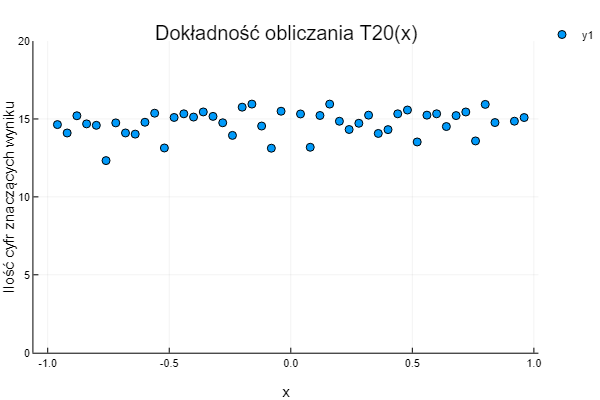
\includegraphics[scale=0.60]{wykres1.png}
\end{center}
Na wykresie widać, że algorytm Clenshawa obliczył wartość $T_{20}(x)$, dla \\ $x \in [-1,1]$ ze średnią dokładnością 15 cyfr znaczących wyniku, co jest zadowalające. 

\subsection{Poprawność numeryczna algorytmu Clenshawa}
\paragraph{Współczynniki $c_{k} := \sqrt{k}$}
Niech $c_{k} := \sqrt{k}$, oraz $\overline{c_{k}} := c_{k} (1 + \epsilon_{k}) $, dla $ \epsilon_{k} \in [-2^{-48}, 2^{-48}]$. Algorytm Clenshawa jest numerycznie poprawny, jeśli wartości sumy  $\sum_{k=0}^{'n} c_{k} T_{k}(x)$ dla dokładnych ($c_{k}$) oraz lekko zaburzonych ($\overline{c_{k}}$) danych będą do siebie zbliżone, czyli jeśli błąd względny tych wartości będzie niewielki. Wykres przedstawia obliczenia dla $n=20$ oraz $x \in [0,10]$, wyniki dla innych wartości $n$ oraz $x$ nie różnią się znacznie od tych przedstawionych poniżej.
\begin{center}
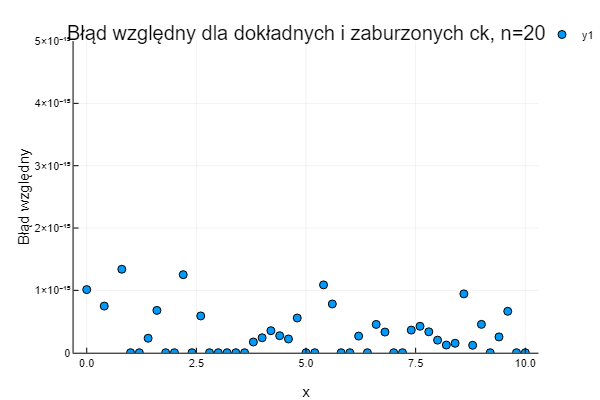
\includegraphics[scale=0.60]{wykres2.png}
\end{center}
Z wykresu widzimy, że błąd względny wyniku jest nie większy, niż $10^{-14}$, a dla niektórych argumentów jest on mniejszy niż precyzja Float64, stąd reprezentowany jest jako $0$. Należy również zauważyć, że wartość zaburzenia współczynników $c_{k}$ jest losowa, a więc i błąd względny wyniku zależy od pewnej losowej wartości.\\
\paragraph{Poprawność numeryczna na przykładzie wielomianów interpolacyjnych}
Powyższe badanie powtórzymy dla sumy z innymi współczynnikami. Niech:
\begin{center}
$t_{n+1,k} = \textrm{cos} \frac{2k+1}{2n+2} \pi$\\
\vspace{0.3em} $I_{n} (x) = \frac{2}{n+1} \sum_{k=0}^{'n} \Bigl( \sum_{i=0}^{n} f(t_{n+1,i}) T_{k}(t_{n+1,i}) \Bigr) T_{k}(x)$\\
\vspace{0.2em} $u_{n-1,k} = \textrm{cos} \frac{k}{n} \pi$ \\
\vspace{0.3em} $J_{n} (x) = \frac{2}{n} \sum_{k=0}^{''n} \Bigl( \sum_{i=0}^{''n} f(u_{n-1,k}) T_{i}(u_{n-1,k}) \Bigr) T_{k}(x)$
\end{center}
Wielomiany $I_{n}(x)$ oraz $J_{n}(x)$ interpolują funkcję $f(x)$ w węzłach Czebyszewa. 
\paragraph{Wielomian $I_{n}(x)$}
Niech $f(x) := x^{22} + x^{7} + e^{x}$. Obliczymy wielomian $I_{n}$ za pomocą algorytmu Clenshawa ze współczynnikami $c_{k} = \sum_{i=0}^{n} f(t_{n+1,i}) T_{k}(t_{n+1,i})$ dla różnych wartości $n$ oraz dla $x$ z różnych przedziałów. Obliczenia powtórzymy dla zaburzonych współczynników $c_{k}$ i sprawdzimy błąd względny tych wartości.
\begin{center}
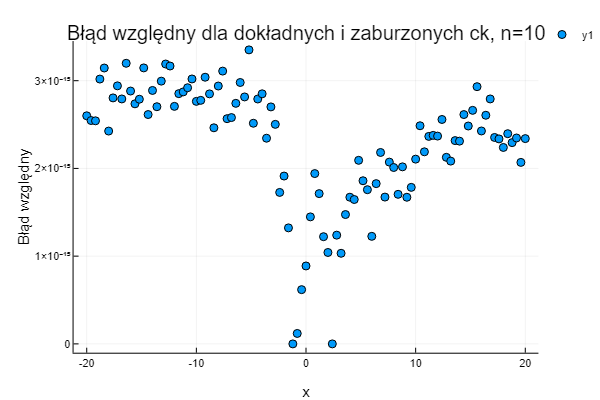
\includegraphics[scale=0.60]{wykres3.png}
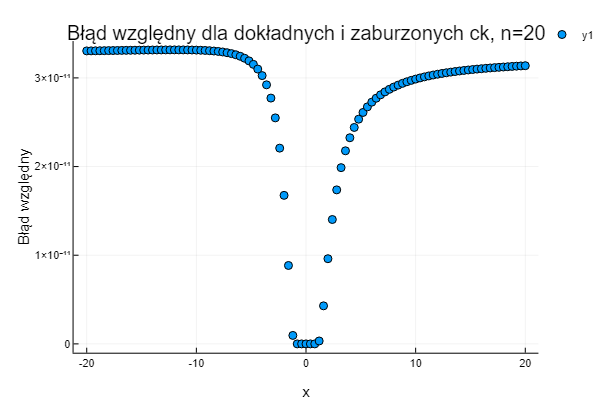
\includegraphics[scale=0.60]{wykres4.png}
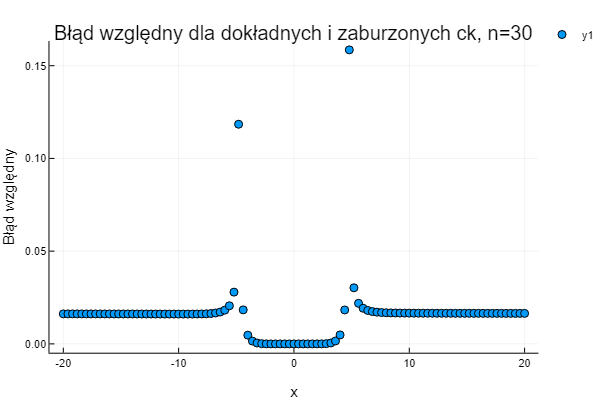
\includegraphics[scale=0.60]{wykres7.png}
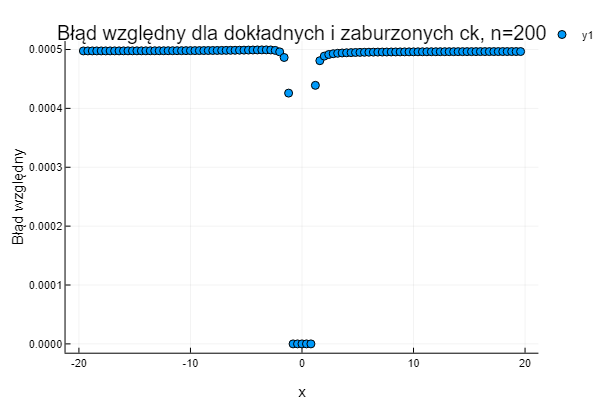
\includegraphics[scale=0.60]{wykres5.png}
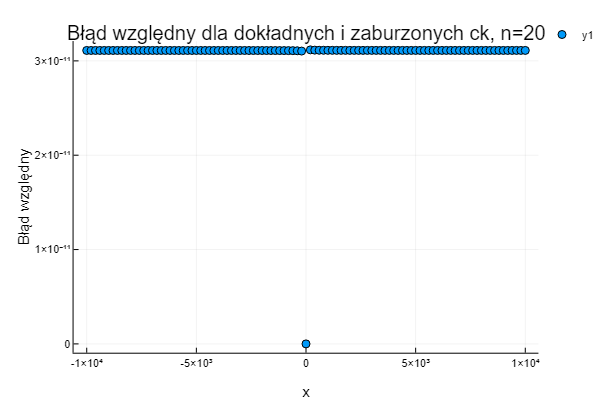
\includegraphics[scale=0.60]{wykres6.png}
\end{center}
Z wykresów widzimy, że niezależnie od wartości $n$ błąd względny obliczeń jest najmniejszy dla $x \in [-5,5]$, dla $x$ spoza tego przedziału błąd względny wyniku nie zmienia się, niezależnie od zmian $x$ (dla zadanej wartości $n$). \\
Większe znaczenie dla błędu względnego wyniku ma zmiana wartości $n$. Dla $n \in [1,20]$ błąd względny wyniku nie przekracza wartości $10^{-10}$, dla $n \in [21,200]$ błąd względny przyjmuje wartości z przedziału $[10^{-4},10^{-1}]$, dla $n > 200$ obliczenie wartości wielomianu $I_{n}(x)$ przestaje być możliwe (otrzymywane wartości są zbyt duże, by na nich operować). Wyniki te utrzymują się dla innych funkcji $f(x)$.

\paragraph{Wielomian $J_{n}(x)$}
Niech $f(x) := x^{22} + x^{7} + e^{x}$. Obliczymy wielomian $J_{n}$ za pomocą algorytmu Clenshawa ze współczynnikami 
\begin{center}
$c_{k} = \sum_{i=0}^{''n} f(u_{n-1,k}) T_{i}(u_{n-1,k}) = \sum_{i=0}^{'n} f(u_{n-1,k}) T_{i}(u_{n-1,k}) - \frac{1}{2} f(u_{n-1,n}) T_{i}(u_{n-1,n})$
\end{center}
Współczynniki $c_{k}$ obliczymy również za pomocą algorytmu Clenshawa.
Obliczenia wykonamy dla różnych wartości $n$ oraz dla $x$ z różnych przedziałów. Obliczenia powtórzymy dla zaburzonych wartości współczynników $c_{k}$ i sprawdzimy błąd względny tych wartości.
\begin{center}
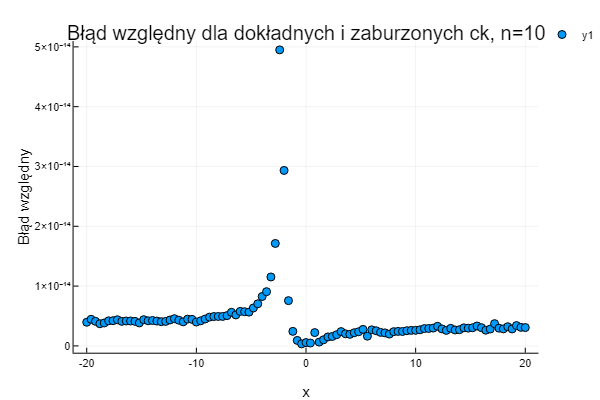
\includegraphics[scale=0.60]{wykres8.png}
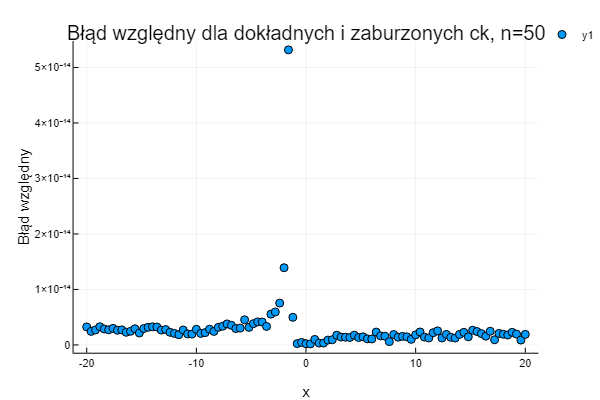
\includegraphics[scale=0.60]{wykres9.png}
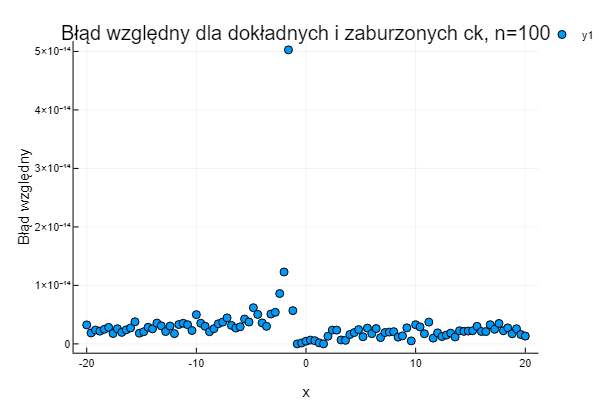
\includegraphics[scale=0.60]{wykres10.png}
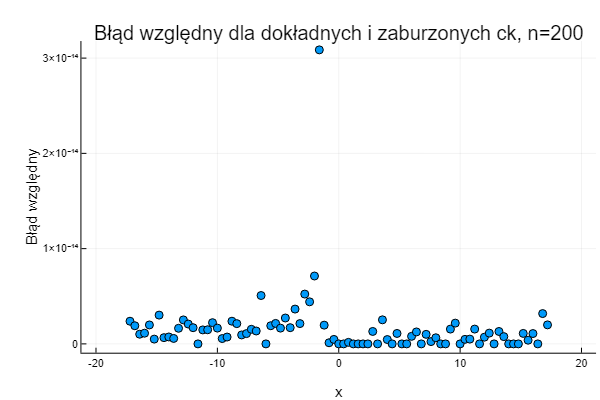
\includegraphics[scale=0.60]{wykres11.png}
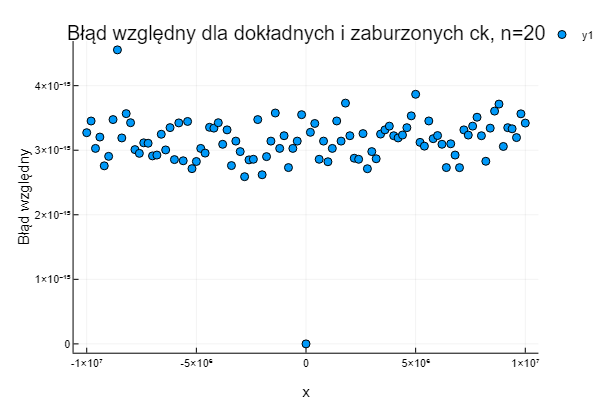
\includegraphics[scale=0.60]{wykres12.png}
\end{center}
Jak widać na wykresach dla $J_{n}(x)$ błąd względny sumy obliczonej za pomocą zaburzonych oraz niezaburzonych współczynników $c_{k}$ nie przekracza $10^{-13}$, niezależnie od $n$ ani od przedziału $x$. Podobnie, jak dla wielomianu $I_{n}(x)$ dla dużych wartości $n$ oraz $x$ wartość wielomianu jest niemożliwa do policzenia. Wyniki te potwierdzają się dla innych funkcji $f(x)$.

\subsection{Wnioski}
Na powyższych przykładach widać, że istnieją takie współczynniki $c_{k}$, które nawet lekko zaburzone powodują, że błąd względny wyniku wynosi $10^{-1}$. Dla wielu innych współczynników algorytm Clenshawa zachowywał poprawność numeryczną. Błąd względny pomiędzy sumą o współczynnikach prawidłowych,\\ a sumą o lekko zaburzonych współczynnikach miał najczęściej wartość rzędu pomiędzy $10^{-15}$, a $10^{-10}$. Jest to zadowalający wynik. Warto również zaznaczyć, że nawet dla skrajnych wartości $n$, czy też $x$ nie udało się uzyskać dużych wartości błędu względnego, co wskazuje na numeryczną poprawność tego algorytmu w większości przypadków.

\section{Podsumowanie}
Wzorując się na algorytmie Clenshawa skonstruowaliśmy skuteczny algorytm do obliczania wartości sum postaci $s_{n}(x) = \sum_{k=0}^{'n} c_{k} T_{k}(x)$. Algorytm ten pozwala wykonać jak najmniej operacji, co gwarantuje nie tylko szybkie działanie, ale również numeryczną poprawność dla większości współczynników $c_{k}$. Z przeprowadzonych eksperymentów widzimy, że błąd względny pomiędzy wartością tej sumy dla poprawnych oraz lekko zaburzonych wartości $c_{k}$ w większości przypadków nie przekracza $10^{-10}$, co jest bardzo dobrym wynikiem.
\section{Literatura}

1) D. Kincaid, W. Cheney, Analiza numeryczna, WNT, 2005.\\

\end{document}
